\documentclass{article}
\usepackage{graphicx} % Required for inserting images
\usepackage[italian]{babel}
\usepackage{amsmath}
\usepackage{amssymb}
\usepackage{algorithm}
\usepackage{algpseudocode}
\usepackage[hidelinks]{hyperref}
\usepackage{svg}

\newtheorem{theorem}{Teorema}

\title{Progettazione di algoritmi}
\author{Leonardo Ganzaroli}
\date{}

\begin{document}

\maketitle

\addcontentsline{toc}{section}{\protect\numberline{}Introduzione}

\tableofcontents

\hypersetup{allcolors=black}

\newpage

\section*{Introduzione}

Questi appunti sono derivanti principalmente dalle slide del corso di \textit{Progettazione di algoritmi} che ho seguito durante la laurea Triennale di informatica all'università "La Sapienza".

\noindent \textbf{N.B. Questo corso è il naturale proseguimento di \textit{Introduzione agli algoritmi}, quindi molte cose saranno date per scontate}.

\newpage

\section{Teoria dei grafi}

\textbf{N.B Se non meglio specificato $|V(G)|=n,|E(G)|=m$.}\newline

\noindent\textbf{Definizione} Un cappio è un arco di un vertice in se stesso.\newline

\noindent\textbf{Definizione} Un multigrafo è un grafo che ammette archi ripetuti e cappi.\newline

\noindent\textbf{Definizione} 2 vertici $x,y$ collegati da un arco sono detti adiacenti, l'arco è detto incidente in $x,y$.\newline

\noindent\textbf{Definizione} Un grafo è detto diretto se i suoi archi hanno un orientamento.\newline

\noindent\textbf{Definizione} Il grado di un vertice ($deg()$) è pari al numero di archi incidenti in esso, se il grafo è diretto si distinguono grado entrante e uscente.\newline

\noindent Per rappresentare un grafo ci sono 2 modi:
\begin{enumerate}
    \item \textbf{Matrice di adiacenza}

        $M\in Matr_{n\times n}(\{0,1\})$ t.c.:

        \[m_{i,j}=
        \begin{cases}
            1\ \text{ se }\ (v_i,v_j)\in E(G)\\
            0\ \text{ altrimenti}
        \end{cases}
        \]
    
    \item \textbf{Liste di adiacenza}

        $\forall\ x\in V(G)$:

        $$L_x=[v\in V(G)\ |\ (x,v),(v,x)\in E(G)]$$

        Se il grafo è diretto ce ne sono 2 per vertice: $L_x^{in},L_x^{out}$.\newline
    
\end{enumerate}

\begin{table}[ht]
    \centering
    \begin{tabular}{c|c|c}
        $(x$ vertice) & \textbf{Matrice} & \textbf{Liste}\\
         \hline
        \rule{0pt}{3ex}\textbf{Spaziale} & $O(n^2)$ & $O(n+m)$\\
         \hline
        \rule{0pt}{3ex}\textbf{Verificare esistenza arco} & $O(1)$ & $O(deg(x))$\\
         \hline
        \rule{0pt}{3ex}\textbf{Trovare adiacenti} & $O(n)$ & $O(deg(x))$\\
         \hline
        \rule{0pt}{3ex}\textbf{Aggiungere/Rimuovere arco} & $O(1)$ & $O(deg(x))$\\
    \end{tabular}
    \caption{Costi}
    \label{tab:costi_grafo}
\end{table}

\noindent\textbf{Definizione} Una traccia è una passeggiata senza archi ripetuti.\newline

\noindent\textbf{Definizione} Una cammino è una traccia senza vertici ripetuti.\newline

\noindent\textbf{Definizione} Una passeggiata è detta chiusa se il primo vertice è anche l'ultimo, altrimenti si dice aperta.\newline

\noindent\textbf{Definizione} Dati $x,y$ vertici. $y$ è visitabile da $x$ ($x\rightarrow y$) se esiste una passeggiata da $x$ a $y$.\newline

\noindent\textbf{Definizione} Una passeggiata è detta Euleriana se contiene tutti gli archi ed ogni arco è presente una sola volta.\newline

\begin{theorem}[Eulero] $\ $\newline
    \[\exists\ \text{ passeggiata Euleriana chiusa }\iff\begin{cases}
        \forall\ v_1,v_2\in V(G)\ \ \exists v_1\rightarrow v_2\\
        \forall\ v\in V(G)\ \ \exists k\in\mathbf{Z}\ |\ deg(v)=2k
    \end{cases}\]\newline
\end{theorem}

\noindent\textbf{Definizione} Un grafo è fortemente connesso se $\forall\ x,y\in V(G)\ \ \exists\ \text{ 2 cammini }\ |\ x\rightarrow y \wedge y\rightarrow x$.\newline

\noindent\textbf{Definizione} Un'arborescenza è un albero diretto.\newline

\noindent I grafi possono essere usati in molti ambiti, un esempio di applicazione è il seguente:

\begin{figure}[ht]
    \centering
    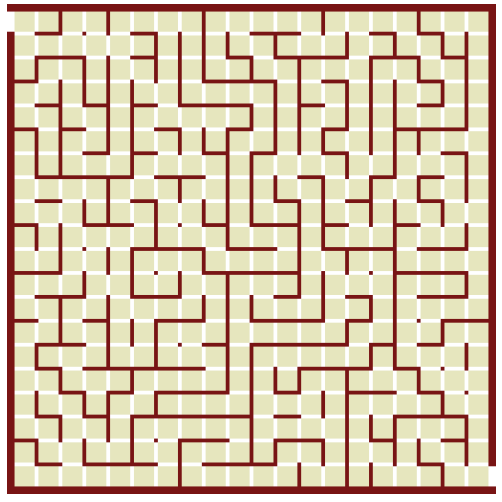
\includegraphics[width=0.4\linewidth]{labr.png}
    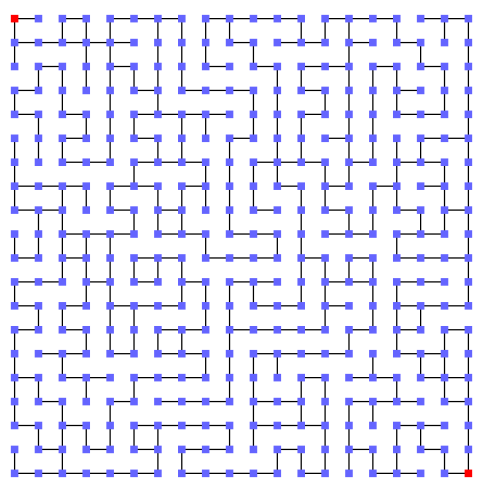
\includegraphics[width=0.4\linewidth]{labr2.png}
    \caption{Labirinto $\rightarrow$ Grafo}
    \label{fig:labr}
\end{figure}

\noindent In questo modo basta trovare un cammino tra l'entrata e l'uscita per attraversarlo.

\newpage

\subsection{Visite}

\begin{algorithm}[ht]
\caption{DFS (Ricorsiva)}
\begin{algorithmic}

\State G grafo, x nodo iniziale
\State

\State Vis = $\{x\}$
\State DFS(G,x,Vis)
\State Return Vis

\State

\Function {DFS}{G,x,Vis}

    \For{$y\in x.$out}
        \If{$y\notin$Vis}

            \State Vis.add($y$)
            \State DFS(G,y,Vis)

        \EndIf
    \EndFor

\EndFunction

\end{algorithmic}
\end{algorithm}

\noindent Il costo è $O(n+m)$, effettua una visita in profondità (simile a quella di un albero).\newline\newline

\begin{algorithm}[ht]
\caption{BFS}
\begin{algorithmic}

\State G grafo, x nodo iniziale
\State

\State Vis = $\{x\}$
\State Q = coda vuota
\State Q.enqueue(x)
\State

\While{$Q\neq\emptyset$}
    \State y = Q.dequeue()

    \For{$z\in y.$out}
    
        \If{$z\notin$Vis}

            \State Q.enqueue($z$)

        \EndIf
    \EndFor
    
\EndWhile

\State
\State Return Vis

\end{algorithmic}
\end{algorithm}

\noindent Il costo è $O(n+m)$, effettua una visita in ampiezza. Inserendo un opportuno array si possono trovare anche le distanze dei nodi da quello iniziale (numero di archi).\newline

\subsection{Studio dei grafi}

\subsubsection{Classificazione archi}

\textbf{Definizione} Dato un contatore $C$ incrementato ad ogni vertice visitato. Se si esegue una DFS si definisce $\ \forall\ x\in V(G)$:
\begin{itemize}
    \item \textbf{Tempo di visita di $x$ } ($t(x)$)

        Valore di $C$ quando $x$ è aggiunto allo stack.

    \item \textbf{Tempo di chiusura di $x$ } ($T(x)$)

        Valore di $C$ quando $x$ è rimosso dallo stack.

    \item \textbf{Intervallo di visita di $x$}

        $$Int(x)=[t(x),T(x)]$$\newline
    
\end{itemize}

\noindent\textbf{Definizione} Data $A$ arborescenza generata da una DFS su $G$ grafo. Si possono usare gli intervalli per catalogare gli archi $(u,v)\in E(G)-E(A)$:
\begin{itemize}
    \item \textbf{All'indietro}

        $$Int(u)\subseteq Int(v)$$
    
    \item \textbf{In avanti}

        $$Int(u)\supseteq Int(v)$$
    
    \item \textbf{Di attraversamento}

        $$Int(u)\cap Int(v)=\emptyset$$\newline
    
\end{itemize}

\begin{theorem}[Cicli]
    $$\exists\text{ ciclo in G}\iff\exists\text{ arco all'indietro in G}$$\newline
\end{theorem}

\noindent\textbf{Definizione} Un ponte è un arco che non appartiene a nessun ciclo.\newline

\subsubsection{Ordinamento}

\textbf{Definizione} Un ordinamento topologico è un ordinamento dei vertici tale che ogni vertice viene prima dei vertici raggiungibili da esso.

\begin{figure}[H]
    \centering
    \includesvg[width=0.4\linewidth]{ord.svg}
    \label{fig:ord}
\end{figure}

\noindent 2 possibili ordinamenti di questo grafo sono:
\begin{enumerate}
    \item 1,2,3,6,4,5,7
    \item 1,2,6,4,3,5,7\newline
\end{enumerate}

\begin{theorem}[Cicli]
    $$\exists\ \text{ ordinamento topologico}\iff \nexists \ \text{ ciclo}$$\newline
\end{theorem}

\begin{algorithm}[ht]
\caption{Trova ordinamento DAG}
\begin{algorithmic}

\State G grafo
\State

\State L = lista vuota
\State

\While{$V(G)\neq\emptyset$}
    \State $v=v\in V(G)\ |\ deg_{out}(v)=0$
    \State L.insert$\_$head(v)
    \State G.remove(v)
\EndWhile

\State
\State Return L

\end{algorithmic}
\end{algorithm}

\noindent Se $G$ è rappresentato con le liste ha costo $O(n(n+m))$.

\subsubsection{Componenti}

\textbf{Definizione} Dato $G$ grafo. Un componente di $G$ è un suo sottografo fortemente connesso e massimale.\newline

\begin{figure}[ht]
    \centering
    \includesvg[width=0.35\linewidth]{comp.svg}
    \label{fig:comp}
\end{figure}

\noindent I componenti di questo grafo sono:
\begin{itemize}
    \item $H_1=\{1,2,3,4\}$
    \item $H_5=\{5,6,8\}$
    \item $\{7\}$\newline
\end{itemize}

\noindent\textbf{Definizione} La contrazione di un componente in un vertice ($G/V(H)$) è l'operazione con cui:
\begin{itemize}
    \item Si rimuovono dal grafo i vertici del componente
    \item Si inserisce un vertice apposito
    \item Si sistemano gli archi\newline
\end{itemize}

\begin{figure}[ht]
    \centering
    \includesvg[width=0.4\linewidth]{comp2.svg}
    \label{fig:comp2}
    \caption{$G/V(H_5)$}
\end{figure}

\section{Algoritmi Greedy}

\textbf{Definizione} Un algoritmo è Greedy se cerca una soluzione ammissibile da un punto
di vista globale attraverso la scelta della soluzione più conveniente ad ogni passo
locale.\newline

\noindent Per questo tipo di algoritmi è sempre necessario dimostrare la correttezza, per farlo si deve:
\begin{enumerate}
    \item Dimostrare che l'output abbia le caratteristiche previste
    \item Dimostrare (con induzione) che ogni istanza di output sia nella soluzione ottimale
    \item Dimostrare che l'output finale sia la soluzione ottimale
\end{enumerate}

\noindent\rule{\textwidth}{0.5pt}

\noindent Si supponga di dover effettuare un viaggio dalla località A alla località B con un'auto che ha un’autonomia di $k$ chilometri e con serbatoio vuoto all'inizio. Lungo la strada ci sono $n + 1$ distributori di benzina ciascuno distante dal precedente meno di $k$ chilometri. Sia $d_i$ la distanza che separa il distributore $i$ dal distributore $i + 1$, dove il distributore 1 è in A e il distributore n + 1 è in B. \newline

\noindent Descrivere un algoritmo greedy che preso in input la lista delle distanze $d_1,\ldots,d_n$ dei distributori, seleziona un numero minimo di distributori in cui far rifornimento durante il viaggio.

\begin{algorithm}[ht]
    \caption{}
    \begin{algorithmic}

        \State d array distanze, k autonomia
    
        \State
        \State R = array di 0
        \State aut = 0
        \For{i=1 to n}

            \If{aut$<$d[i]}

                \State aut = k
                \State R[i] = 1
            
            \EndIf

            \State aut -= d[i]
            
        \EndFor

        \State Return R
        
    \end{algorithmic}
\end{algorithm}

\begin{itemize}
    \item Grazie all'IF ogni soluzione prodotta è ammissibile
    \item Induzione

        Base: $i=0$, niente da provare

        Sia $R_i$ l'array $R$ dopo l'$i$-esima iterazione, $R^*$ la soluzione ottima.

        Per ipotesi fino ad $i$ coincidono, analizzo i casi non coincidenti in $i+1$:
        \begin{enumerate}
            \item $R_{i+1}[i+1]=1\wedge R^*[i+1]=0$

                Non può essere $i+1=n+1$ perché ci sono massimo $n$ iterazioni e R non avrebbe 1 in quella posizione.

                Se $i+1<n+1$ il fatto che venga scelto il distributore $i+1$ implica che l'autonomia non basti per arrivare a $i+2$, la soluzione sarebbe quindi sbagliata.

            \item $R_{i+1}[i+1]=0\wedge R^*[i+1]=1$

                Non può essere $i+1=n+1$ altrimenti la soluzione avrebbe un rifornimento di troppo. 
                
                Se $i+1<n+1$ il fatto che non venga scelto implica che c'è abbastanza autonomia per arrivare a $i+2$, quindi la soluzione avrebbe un rifornimento di troppo.
            
        \end{enumerate}
    
\end{itemize}

\noindent\rule{\textwidth}{0.5pt}

\subsection{Grafi pesati}

\textbf{Definizione} Un grafo pesato è un grafo in cui ogni arco ha associato un valore reale.\newline

\noindent\textbf{Definizione} Il peso di un cammino ($p()$) è la somma dei pesi degli archi del cammino.\newline

\noindent\textbf{Definizione} La distanza pesata tra 2 vertici $x,y$ ($dist(x,y)$) è il cammino tra i 2 con peso minimo.
    
\begin{algorithm}[ht]
    \caption{Dijkstra (Grafo non diretto)}
    \begin{algorithmic}
        \State dist = array di $+\infty$
        \State Padri = array di -1
        \State dist[$u$] = 0 \Comment{$u$ nodo iniziale}
        \State Padri[$u$] = $u$
        \State $H$ = min-Heap \Comment{inizializzato con tutti i nodi, priorità=dist}

        \While{$H\neq\emptyset$}

            \State v = $H.$get\_min() \Comment{Rimuovi il nodo minore}

            \For{$w\in v.$out}

                \If{$dist[w]>dist[v]+p[v,w]$}

                    \State $dist[w]=dist[v]+p(v,w)$
                    \State Padri[$w$] = $v$
                    \State Aggiorna $H$

                \EndIf
                    
            \EndFor

        \EndWhile

        \State Return dist,Padri
        
    \end{algorithmic}
\end{algorithm}

\noindent Il costo è $O((n+m)\log n)$.

\subsubsection{MST}

\noindent\textbf{Definizione} Un sottografo di un grafo connesso e non diretto è un albero di copertura se è aciclico e contiene tutti i nodi del grafo.\newline

\noindent\textbf{Definizione} L'albero di copertura minima di un grafo (MST) è il suo albero di copertura la cui somma degli archi è la minima.\newline

\begin{algorithm}[ht]
    \caption{Kruskal}
    \begin{algorithmic}

    \State Sol = $\emptyset$

    \State Sort($E(G)$)

    \For{$e\in E(G)$}

        \If{Trova\_ciclo($\text{Sol}\cup e$)==$\emptyset$}

            \State Sol.add($e$)

        \EndIf
            
    \EndFor

    \State Return Sol
        
    \end{algorithmic}
\end{algorithm}

\begin{algorithm}[ht]
    \caption{Prim}
    \begin{algorithmic}

    \State $v$ = $v\in V(G)$
    \State Sol = $\emptyset$
    \State R = $\{v\}$

    \While{R$\neq V(G)$}

        \State $(x,y)=min[w(a,b)]$ con $a\in R\wedge b\in V(G)-R$
        \State Sol.add($(x,y)$)
        \State R.add($y$)
            
    \EndWhile

    \State Return Sol
        
    \end{algorithmic}
\end{algorithm}

\noindent Entrambi ritornano un MST del grafo, il costo è $O(mn)$ per entrambi.\newline

\newpage

\section{Programmazione dinamica}

\textbf{Definizione} La programmazione dinamica è basata sulla risoluzione
di un problema partendo dalle soluzioni dello stesso problema ma di dimensione inferiore.\newline

\noindent\textbf{Definizione} La memoization consiste nel salvare in memoria i valori dati da una funzione per poterli usare successivamente senza ricalcolarli, si può usare solo se la funzione non ha effetti collaterali e dà sempre lo stesso output con un certo input.\newline

\noindent Per fare ciò si usa una matrice.\newline

\noindent\rule{\textwidth}{0.5pt}
Esempi:
\begin{itemize}
    \item \textbf{Knapsack Problem}
    
            Dati degli oggetti $x_1,\ldots,x_n$ ognuno con un suo peso $w_i$ ed un suo valore $v_i$ trovare un sottoinsieme che massimizzi il valore totale tenendo il peso sotto la soglia $W$.\newline
    
            Si definisce la tabella $T$ di dimensione $n+1\times W+1$ tale che:
    
            $$T[k,x]=(\text{max valore trasportabile con uno zaino di capacità $x\leq W$ con i primi $k$ oggetti})$$\newline
    
            Nello specifico:
    
            \[T[k,x]=\begin{cases}
                0 & \text{ se } x=0\vee k=0\\
                T[k-1,x]& \text{ se } w_k>x\\
                max(T[k-1,x],T[k-1,x-w_k]+v_k)& \text{ se } w_k\leq x
            \end{cases}\]\newline
    
    
            Per trovare la soluzione basta partire dalla cella in basso a destra e risalire una riga alla volta, nel caso $T[k,x]>T[k-1,x]$ si aggiunge l'elemento corrente alla soluzione e ci si sposta verso sinistra di $w_k$ colonne.

    \newpage

    \item \textbf{Cammino peso max}

            Dato un DAG pesato e due vertici $x,y$ trovare il cammino con peso massimo tra i 2.\newline
    
            Essendo un DAG con $n$ vertici ci sono massimo $n-1$ archi, si definisce quindi la tabella $n\times n$ tale che:
    
            $$T[k,z]=(\text{peso max del cammino $x\rightarrow z$ passante per max $k$ archi})$$\newline
    
            Nello specifico:
            \begin{itemize}
                \item $T[0,x]=0$
                \item $\forall\ z\neq x\ \ T[0,z]=-\infty$
                \item $\forall\ k\in[0,n-1]\ \ T[k,z]=-\infty$ se $\nexists$ cammino $x\rightarrow z$ lungo $k$
                \item $T[1,z]=w(x,z)$ se $\exists(x,z)\in E(G)$, $T[0,z]$ altrimenti\newline
            \end{itemize}
    
            Quindi:
    
            $$T[k,z]=max(T[k-1,z],T[k-1,v_1]+w(v_1,z),\ldots,T[k-1,v_h]+w(v_h,z))$$\newline
    
            Il cammino si trova con procedimento simile al precedente.

        \item \textbf{CPM}

            Un progetto si può dividere in attività $1,2,\ldots,n$, ogni attività ha un suo tempo di svolgimento e possono esistere dipendenze tra 2 attività. Si vogliono sapere i tempi di inizio delle attività ed il tempo totale necessario.\newline

            Si segue il procedimento:
            \begin{enumerate}
                \item Costruire un DAG i cui nodi sono le attività e gli archi le dipendenze, il peso di quest'ultime è il tempo di esecuzione del nodo di partenza
                \item Aggiungere un nodo \textit{Start} con archi uscenti ad ogni altro nodo con costo 0
                \item Il cammino con peso maggiore da \textit{Start} ad un certo nodo fornisce il tempo di inizio per lo stesso
                \item Il tempo totale è dato dal costo del cammino massimo all'ultimo nodo + il suo tempo di completamento
            \end{enumerate}

        \newpage

        \item \textbf{Bellman-Ford}

            Trovare il cammino minimo tra 2 nodi in presenza di costi negativi (no cicli negativi).\newline

            Come visto in precedenza:

            $$T[k,z]=(\text{peso min cammino $x\rightarrow z$ passante per max $k$ archi})$$\newline

            Nello specifico:
            \begin{itemize}
                \item $T[0,x]=0$
                \item $\forall\ z\neq x\ \ T[0,z]=+\infty$
                \item $\forall\ k\in[0,n-1]\ \ T[k,z]=+\infty$ se $\nexists$ cammino $x\rightarrow z$ lungo $k$
                \item $T[1,z]=w(x,z)$ se $\exists(x,z)\in E(G)$, $T[0,z]$ altrimenti\newline
            \end{itemize}

            Quindi:
    
            $$T[k,z]=min(T[k-1,z],T[k-1,v_1]+w(v_1,z),\ldots,T[k-1,v_h]+w(v_h,z))$$
    
\end{itemize}


\noindent\rule{\textwidth}{0.5pt}

\end{document}
